\documentclass[11pt]{article}

\usepackage[T1]{fontenc}
\usepackage[utf8]{inputenc}
\usepackage{lmodern}
\usepackage{microtype}
\usepackage[a4paper,margin=27mm]{geometry}
\usepackage{amsmath,amssymb,mathtools,amsthm}
\usepackage{booktabs,tabularx,array,longtable}
\usepackage{graphicx}
\usepackage{enumitem}
\usepackage{xcolor}
\usepackage{hyperref}
\usepackage[nameinlink,capitalize,noabbrev]{cleveref}
\usepackage{listings}
\usepackage{fancyhdr}
\usepackage{caption}
\usepackage{subcaption}
\usepackage{url}

\hypersetup{
  colorlinks=true,
  linkcolor=blue!55!black,
  citecolor=green!40!black,
  urlcolor=blue!60!black,
  pdfauthor={OpenAI GPT-5.6 Pro},
  pdftitle={Finite dyadic sinc products and piecewise-polynomial approximants to Rvachev's up-function}
}

\pagestyle{fancy}
\fancyhf{}
\fancyhead[L]{\small Finite dyadic sinc products}
\fancyhead[R]{\small\nouppercase{\leftmark}}
\fancyfoot[C]{\thepage}
\setlength{\headheight}{14pt}

\newtheorem{theorem}{Theorem}[section]
\newtheorem{proposition}[theorem]{Proposition}
\newtheorem{lemma}[theorem]{Lemma}
\newtheorem{corollary}[theorem]{Corollary}
\newtheorem{conjecture}[theorem]{Conjecture}
\newtheorem{problem}[theorem]{Problem}
\theoremstyle{definition}
\newtheorem{definition}[theorem]{Definition}
\newtheorem{example}[theorem]{Example}
\theoremstyle{remark}
\newtheorem{remark}[theorem]{Remark}

\newcommand{\R}{\mathbb R}
\newcommand{\N}{\mathbb N}
\newcommand{\E}{\mathbb E}
\newcommand{\Pp}{\mathbb P}
\newcommand{\Var}{\operatorname{Var}}
\newcommand{\supp}{\operatorname{supp}}
\newcommand{\Up}{\operatorname{up}}
\newcommand{\sinc}{\operatorname{sinc}}
\newcommand{\wt}{\operatorname{wt}}
\newcommand{\dd}{\,\mathrm d}
\newcommand{\pos}[1]{\left(#1\right)_{+}}
\newcommand{\norm}[1]{\left\lVert #1\right\rVert}
\newcommand{\abs}[1]{\left\lvert #1\right\rvert}
\newcommand{\qpoch}[2]{\left(#1;#2\right)}
\newcommand{\qbinom}[3]{\genfrac{[}{]}{0pt}{}{#1}{#2}_{#3}}
\newcommand{\e}{\mathrm e}
\newcommand{\ii}{\mathrm i}
\newcommand{\Fourier}{\mathcal F}
\newcommand{\tm}{\tau}
\newcommand{\deltaN}{\delta_n}
\newcommand{\AN}{A_n}

\definecolor{shade}{gray}{0.95}
\lstdefinestyle{reportcode}{
  basicstyle=\ttfamily\small,
  backgroundcolor=\color{shade},
  frame=single,
  columns=fullflexible,
  keepspaces=true,
  showstringspaces=false,
  breaklines=true,
  xleftmargin=0.5em,
  xrightmargin=0.5em
}

\title{\bfseries Finite Dyadic Sinc Products and Piecewise-Polynomial\\
Approximants to Rvachev's Up-Function\\[0.5em]
\large Exact splines, sharp convergence laws, Bell--Bernoulli expansions,\\
and positive quadrature acceleration}
\author{Research report prepared from the \texttt{ProveIt} Fabius-function documentation\\
\small Computational supplement: \texttt{finite\_sinc\_experiments.py}}
\date{28 August 2026}

\begin{document}
\maketitle

\begin{abstract}
Let
\[
 \Phi(\xi)=\widehat{\Up}(\xi)
 =\prod_{j=0}^{\infty}\sinc\!\left(\frac{\pi\xi}{2^j}\right),
 \qquad \sinc z=\frac{\sin z}{z},
\]
under the Fourier convention
$\widehat f(\xi)=\int_{\R}f(x)\e^{-2\pi\ii x\xi}\dd x$.
This report studies the inverse transforms $p_n$ of the first $n$ factors.
They are nonstationary dyadic box splines: compactly supported, nonnegative,
even, log-concave, piecewise polynomial of degree $n-1$, and $C^{n-2}$.
Their knots unexpectedly form a uniform dyadic grid, while the jumps of the
top derivative carry the signed Thue--Morse sequence.  An explicit truncated-power
formula, exact cell formulas, recursions, Fourier-zero multiplicities, partition-of-unity
identities, cumulants, and sharp derivative geometry are obtained.

The main convergence result is an exact law, not merely an upper bound.  For every
$r\ge0$ and $n\ge r+3$,
\[
 \norm{p_n^{(r)}-\Up^{(r)}}_{\infty}
 =\frac{2^{\binom{r+3}{2}-1}}{9\,4^n}.
\]
The extremum occurs at an explicit dyadic point.  The associated distribution
functions satisfy the exact Kolmogorov law $d_K=1/(9\,4^n)$.  At all orders,
$p_n$ admits a uniform differential expansion whose coefficients are complete Bell
polynomials in Bernoulli-number data from $1/\Phi$; geometric Richardson combinations
then give signed $4^{-Mn}$ extrapolation with uniformly bounded coefficient variation.

A second, positive acceleration theory is developed from a new uniform-scale-mixture
representation of $\Up$.  The exact tail is a mixture of uniform boxes governed by a
probability measure $\nu$ on $[0,1]$.  Positive Gauss, Radau, and Lobatto quadrature for
$\nu$ turns the continuum tail into finite positive mixtures of boxes.  A one-signed
Peano-kernel argument and the dyadic derivative plateaux give exact $C^r$ errors for the
whole hierarchy.  In particular, a single variance-matched extra box yields an exact
$16^{-n}$ law, resolving a positive variance-matching direction left open in the
repository's frontier volume; right-Radau rules preserve the exact support $[-1,1]$
and attain arbitrarily high algebraic orders.  Reproducible FFT and exact-rational
experiments verify the formulas to numerical precision.
\end{abstract}

\tableofcontents
\newpage

\section{Scope, source audit, and novelty boundary}
\label{sec:scope}

\subsection{Documents examined}

The source audit covered the living TeX documents under
\path{Analysis/FabiusFunction/docs}, especially the primary synthesis
\emph{The Fabius Function and Rvachev's Up-Function}, the mathematical glossary,
the Lean walkthrough, and the consolidated volume
\emph{Non-formalized Research Frontiers}.  The recursive archive index was also
examined to identify the historical TeX families: early notes, standalone studies,
primary-exposition drafts, supplements, $q$-calculus articles, Lean walkthroughs,
glossaries, and per-topic frontier dossiers.  The archive explicitly records frozen
first-introduced versions and prunes byte-identical copies already present in the live
tree, so the living consolidated sources are the appropriate mathematical baseline
for avoiding duplication \cite{proveit-primary,proveit-frontiers,proveit-archive}.

The existing corpus already develops the probability law of $\Up$, the infinite sinc
product, exact dyadic arithmetic, Thue--Morse identities, derivative tilings, moments,
$q$-binomial structure, endpoint Lambert--$W$ asymptotics, and a repeated-integration
spline $f_n$.  In particular, the frontier volume proves a sharp error law for $f_n$
and explicitly contrasts it with the ordinary prefix density $p_n$, whose sharp law is
not studied there.  It then asks for a positive compactly supported tail replacement
with matching variance, predicting a possible $16^{-n}$ rate but asserting no such
scheme \cite{proveit-frontiers}.

\subsection{What is new here}

The principal additions of this report are:
\begin{enumerate}[leftmargin=2.1em]
\item the exact uniform-grid truncated-power representation of the ordinary inverse
      transform $p_n$, with Thue--Morse jump weights;
\item a sharp derivative-plateau theorem for $p_n$;
\item the exact $C^r$ prefix error law and exact Kolmogorov distance;
\item a uniform all-orders expansion of $p_n$ in even derivatives of $\Up$, with
      Bell--Bernoulli coefficient formulas;
\item stable $q=1/4$ Richardson weights and their closed $q$-binomial form;
\item a uniform-scale-mixture representation of the exact tail;
\item a general positive quadrature theorem giving exact error constants for Gauss,
      Radau, and Lobatto tail surrogates;
\item explicit positive fourth- and sixth-order schemes, including exact-support
      accelerants.
\end{enumerate}
Every theorem below is accompanied by a mathematical proof.  These results have not
been added to the repository's Lean development and should therefore be read as a
research contribution awaiting independent review and formalization.  Numerical
experiments are used as verification, never as a substitute for proof.

\section{Fourier normalization and the probabilistic head--tail model}
\label{sec:model}

\subsection{The infinite product}

We use
\begin{equation}
 \widehat f(\xi)=\int_{\R} f(x)\e^{-2\pi\ii x\xi}\dd x,
 \qquad
 f(x)=\int_{\R}\widehat f(\xi)\e^{2\pi\ii x\xi}\dd\xi.
 \label{eq:fourier-convention}
\end{equation}
For $a>0$, define the centered uniform density
\begin{equation}
 u_a(x)=\frac{1}{2a}\mathbf 1_{[-a,a]}(x).
 \label{eq:uniform-density}
\end{equation}
Then
\begin{equation}
 \widehat{u_a}(\xi)=\sinc(2\pi a\xi).
 \label{eq:uniform-transform}
\end{equation}
Rvachev's normalized up-function is the even $C^\infty$ probability density on
$[-1,1]$ whose transform is
\begin{equation}
 \Phi(\xi)=\widehat\Up(\xi)
 =\prod_{j=0}^{\infty}\sinc\!\left(\frac{\pi\xi}{2^j}\right).
 \label{eq:infinite-product}
\end{equation}
This normalization agrees with the compactly supported function studied by Rvachev
and Arias de Reyna \cite{rvachev1990,arias1982}.

\subsection{Partial products and random sums}

For $n\ge1$, set
\begin{equation}
 \Phi_n(\xi)=\prod_{j=0}^{n-1}\sinc\!\left(\frac{\pi\xi}{2^j}\right),
 \qquad p_n=\Fourier^{-1}\Phi_n.
 \label{eq:prefix-product}
\end{equation}
By \cref{eq:uniform-transform},
\begin{equation}
 p_n=u_{2^{-1}}*u_{2^{-2}}*\cdots*u_{2^{-n}}.
 \label{eq:prefix-convolution}
\end{equation}
Let $U_0,U_1,\ldots$ be independent $\operatorname{Unif}[-1,1]$ variables and put
\begin{equation}
 S_n=\sum_{j=0}^{n-1}2^{-j-1}U_j,
 \qquad
 X=\sum_{j=0}^{\infty}2^{-j-1}U_j.
 \label{eq:random-sums}
\end{equation}
Then $p_n$ is the density of $S_n$ and $\Up$ is the density of $X$.
Introduce
\begin{equation}
 \delta_n=2^{-n},\qquad A_n=1-2^{-n}.
 \label{eq:delta-A}
\end{equation}
The omitted tail is a scaled independent copy of the whole sum:
\begin{equation}
 X\overset d=S_n+\delta_nX',
 \qquad X'\overset d=X,
 \qquad X'\ \text{independent of }S_n.
 \label{eq:head-tail-random}
\end{equation}
Consequently,
\begin{equation}
 \Phi(\xi)=\Phi_n(\xi)\Phi(\delta_n\xi),
 \qquad
 \Up=p_n*\rho_{\delta_n},
 \qquad
 \rho_\delta(x)=\delta^{-1}\Up(x/\delta).
 \label{eq:head-tail-fourier}
\end{equation}
The identity \cref{eq:head-tail-fourier} is the engine behind both the exact error law
and all-order acceleration.

\section{Exact inverse transforms: dyadic box splines with Thue--Morse knots}
\label{sec:exact-spline}

\subsection{Uniform knot formula}

Write
\begin{equation}
 \tau_k=(-1)^{s_2(k)},
 \label{eq:tm-sign}
\end{equation}
where $s_2(k)$ is the binary digit sum.  For $m=0$, the convention
$y_+^0=\mathbf 1_{(0,\infty)}(y)$ is used away from knots.

\begin{theorem}[Exact truncated-power formula]
\label{thm:truncated-power}
For every $n\ge1$,
\begin{equation}
 \boxed{
 p_n(x)=\frac{2^{n(n-1)/2}}{(n-1)!}
 \sum_{k=0}^{2^n-1}\tau_k
 \left(x+A_n-\frac{k}{2^{n-1}}\right)_+^{n-1}.}
 \label{eq:truncated-power}
\end{equation}
The knots are the uniformly spaced points
\begin{equation}
 t_{n,k}=-A_n+\frac{k}{2^{n-1}},
 \qquad 0\le k<2^n.
 \label{eq:knots}
\end{equation}
In distributions,
\begin{equation}
 D^np_n=2^{n(n-1)/2}\sum_{k=0}^{2^n-1}\tau_k\,\delta_{t_{n,k}}.
 \label{eq:top-distributional-derivative}
\end{equation}
\end{theorem}

\begin{proof}
For one box,
\[
 Du_a=\frac{1}{2a}(\delta_{-a}-\delta_a).
\]
Convolving the $n$ derivatives in \cref{eq:prefix-convolution} gives a signed atomic
measure.  Choose a binary vector $b=(b_0,\ldots,b_{n-1})\in\{0,1\}^n$; its atom lies at
\[
 -A_n+\sum_{j=0}^{n-1}b_j2^{-j}
 =-A_n+\frac{k}{2^{n-1}},
 \quad
 k=\sum_{j=0}^{n-1}b_j2^{n-1-j},
\]
and its sign is $(-1)^{\sum b_j}=\tau_k$.  The normalization is
\[
 \prod_{j=0}^{n-1}\frac{1}{2\cdot2^{-j-1}}
 =\prod_{j=0}^{n-1}2^j=2^{n(n-1)/2}.
\]
This proves \cref{eq:top-distributional-derivative}.  Integrating $n$ times from
$-\infty$, using compact support, gives \cref{eq:truncated-power}.
\end{proof}

The equal spacing is special to the dyadic weights.  The $2^n$ subset sums of
$1,1/2,\ldots,2^{1-n}$ fill a complete integer grid after multiplication by
$2^{n-1}$, while their parity signs are exactly Thue--Morse.  Thus a nonstationary
convolution of boxes of different widths becomes a uniform-knot spline with highly
structured signed top derivative.

\subsection{Cell formula and exact arithmetic}

Set
\begin{equation}
 y=2^{n-1}(x+A_n).
 \label{eq:cell-coordinate}
\end{equation}
Inside the support, \cref{eq:truncated-power} becomes
\begin{equation}
 p_n(x)=\frac{2^{-(n-1)(n-2)/2}}{(n-1)!}
 \sum_{0\le k\le\lfloor y\rfloor}\tau_k(y-k)^{n-1}.
 \label{eq:scaled-cell-formula}
\end{equation}
This has several immediate consequences.

\begin{corollary}[Piecewise-polynomial and arithmetic structure]
\label{cor:piecewise-arithmetic}
The function $p_n$ is supported on $[-A_n,A_n]$, is polynomial of degree at most
$n-1$ on each of the $2^n-1$ open knot cells, and belongs to $C^{n-2}(\R)$ for
$n\ge2$.  At rational arguments it has rational values; at dyadic arguments all
computations may be performed with integers after one global power-of-two scaling.
\end{corollary}

On the cell $(t_{n,J},t_{n,J+1})$,
\begin{equation}
 p_n^{(n-1)}(x)=2^{n(n-1)/2}\sum_{k=0}^{J}\tau_k.
 \label{eq:top-cell-value}
\end{equation}
The elementary Thue--Morse prefix identity
\begin{equation}
 \sum_{k=0}^{J}\tau_k=
 \begin{cases}
   \tau_{J/2},&J\text{ even},\\
   0,&J\text{ odd}
 \end{cases}
 \label{eq:tm-prefix}
\end{equation}
therefore shows that every second top-derivative cell is identically zero, while the
remaining cells carry a compressed Thue--Morse pattern.

\subsection{Convolution and scaling recursions}

Appending the final box in \cref{eq:prefix-convolution} gives
\begin{align}
 p_n(x)
 &=2^{n-1}\int_{x-2^{-n}}^{x+2^{-n}}p_{n-1}(t)\dd t,
 \label{eq:last-box-recursion}\\
 p_n'(x)
 &=2^{n-1}\bigl(p_{n-1}(x+2^{-n})-p_{n-1}(x-2^{-n})\bigr).
 \label{eq:last-box-derivative}
\end{align}
The product shell
$\Phi_n(\xi)=\sinc(\pi\xi)\Phi_{n-1}(\xi/2)$ yields the equivalent dilation recursion
\begin{align}
 p_n(x)&=\int_{2x-1}^{2x+1}p_{n-1}(s)\dd s,
 \label{eq:scale-recursion}\\
 p_n'(x)&=2\bigl(p_{n-1}(2x+1)-p_{n-1}(2x-1)\bigr).
 \label{eq:scale-derivative}
\end{align}
These formulas permit exact construction of all cell polynomials by repeated primitive
and shift operations.  They avoid the severe cancellation that can occur in the global
truncated-power sum for large $n$.

\section{Structural properties of the finite-product splines}
\label{sec:properties}

\subsection{Shape, plateau, and partition of unity}

\begin{proposition}[Basic geometry]
\label{prop:basic-geometry}
For every $n\ge1$:
\begin{enumerate}[label=(\roman*),leftmargin=2.1em]
\item $p_n\ge0$, $p_n$ is even, and $\int p_n=1$;
\item $\supp p_n=[-A_n,A_n]$;
\item $p_n$ is log-concave and therefore unimodal;
\item $p_n(x)=1$ for $|x|\le\delta_n$;
\item for $n\ge2$,
\begin{equation}
 \sum_{m\in\mathbb Z}p_n(x-m)=1,
 \qquad
 p_n(x)+p_n(1-x)=1\quad(0\le x\le1).
 \label{eq:partition-unity}
\end{equation}
\end{enumerate}
\end{proposition}

\begin{proof}
The first three assertions follow from convolution of centered uniform densities;
log-concavity is preserved by convolution.  For the plateau, split off the largest box
$u_{1/2}$.  The remaining convolution is supported on
$[-1/2+\delta_n,1/2-\delta_n]$.  If $|x|\le\delta_n$, the interval
$[x-1/2,x+1/2]$ contains that support, so convolution with $u_{1/2}$ integrates the
entire remaining density and equals $1$.

At every nonzero integer $k$, the factor $\sinc(\pi\xi)$ gives $\Phi_n(k)=0$, while
$\Phi_n(0)=1$.  Poisson summation therefore gives the first identity in
\cref{eq:partition-unity}.  On $[0,1]$, the support radius is less than $1$, so only the
translates $m=0,1$ survive; evenness converts $p_n(x-1)$ to $p_n(1-x)$.
\end{proof}

\subsection{Fourier zeros}

Let $v_2(k)$ denote the exponent of $2$ in a nonzero integer $k$.

\begin{proposition}[Exact zero multiplicities]
\label{prop:zero-multiplicity}
For $k\in\mathbb Z\setminus\{0\}$,
\begin{equation}
 \operatorname{ord}_{\xi=k}\Phi_n
 =1+\min\{v_2(k),n-1\}.
 \label{eq:zero-multiplicity}
\end{equation}
For fixed $k$, this stabilizes to $1+v_2(k)$, the multiplicity of the corresponding
zero of $\Phi$.
\end{proposition}

This $2$-adic spectral stratification is the Fourier counterpart of the Thue--Morse
jump pattern.  It also explains why the splines reproduce constants by integer
translation, while higher-order cancellation appears selectively on dyadic frequency
sublattices.

\subsection{Cumulants and the variance defect}

Let $B_{2m}$ be the Bernoulli numbers with $B_2=1/6$ and $B_4=-1/30$.
The even cumulants of $X$ are
\begin{equation}
 \kappa_{2m}(X)=\frac{B_{2m}}{2m(1-2^{-2m})},
 \qquad \kappa_{2m+1}(X)=0.
 \label{eq:cumulants-X}
\end{equation}
Indeed, a uniform $U\sim\operatorname{Unif}[-1,1]$ has
$\kappa_{2m}(U)=2^{2m}B_{2m}/(2m)$, and the geometric weights sum exactly.
From \cref{eq:head-tail-random},
\begin{equation}
 \kappa_{2m}(S_n)=(1-\delta_n^{2m})\kappa_{2m}(X).
 \label{eq:cumulants-prefix}
\end{equation}
In particular,
\begin{equation}
 \E X^2=\frac19,
 \qquad
 \E X^4=\frac{19}{675},
 \qquad
 \E X^6=\frac{583}{59535},
 \label{eq:central-moments}
\end{equation}
and
\begin{equation}
 \Var X-\Var S_n=\frac{\delta_n^2}{9}.
 \label{eq:variance-defect}
\end{equation}
The raw prefix's leading $4^{-n}$ error is exactly this missing variance transported
through the second derivative.

\subsection{Sharp derivative plateaux}

Define
\begin{equation}
 c_m=1-2^{-m}\quad(m\ge0),
 \qquad c_0=0.
 \label{eq:cm}
\end{equation}
The living primary exposition proves the corresponding sharp derivative norm for
$\Up$ through its exact dyadic derivative tiling \cite{proveit-primary}.  The finite
splines possess a stronger local plateau.

\begin{theorem}[Finite-prefix derivative geometry]
\label{thm:derivative-plateau}
Fix $m\ge0$ and $n\ge m+1$.  Interpreting the top derivative at the limiting case
$n=m+1$ as its canonical almost-everywhere step representative, one has
\begin{equation}
 \norm{p_n^{(m)}}_{L^\infty}=2^{\binom{m+1}{2}}.
 \label{eq:pn-derivative-norm}
\end{equation}
Moreover,
\begin{equation}
 p_n^{(m)}(x)=(-1)^m2^{\binom{m+1}{2}}
 \qquad
 \text{for almost every }x\in[c_m-\delta_n,c_m+\delta_n].
 \label{eq:derivative-plateau}
\end{equation}
For $n\ge m+2$ the derivative is classical and the equality holds pointwise on the
closed interval.  By evenness, the reflected plateau has the corresponding parity sign.
\end{theorem}

\begin{proof}
Factor
\[
 p_n=p_{m+1}*q_{m+1,n},
\]
where $q_{m+1,n}$ is the convolution of the remaining boxes and is a probability
density supported on
\[
 \left[-2^{-m-1}+\delta_n,\;2^{-m-1}-\delta_n\right].
\]
By \cref{eq:top-cell-value,eq:tm-prefix}, the step function
$p_{m+1}^{(m)}$ takes only the values
$0$ and $\pm2^{\binom{m+1}{2}}$.  Convolution with a probability measure cannot
increase its supremum norm, proving the upper bound.

The point $c_m$ is the midpoint of the rightmost nonzero cell of
$p_{m+1}^{(m)}$, whose half-width is $2^{-m-1}$.  Translating the support of
$q_{m+1,n}$ across any $x\in[c_m-\delta_n,c_m+\delta_n]$ remains inside that cell.
Hence the convolution averages a constant and gives \cref{eq:derivative-plateau},
which also proves sharpness.
\end{proof}

\section{Sharp convergence of the ordinary partial products}
\label{sec:sharp-convergence}

\subsection{Smooth-test and transport estimates}

The coupling \cref{eq:head-tail-random} immediately gives, for $1\le p<\infty$,
\begin{equation}
 W_p(\mathcal L(S_n),\mathcal L(X))
 \le \delta_n\bigl(\E|X|^p\bigr)^{1/p}\le\delta_n.
 \label{eq:wasserstein-bound}
\end{equation}
The mean-zero tail improves smooth tests by one full power.  If
$\varphi\in C^2(\R)$ has bounded second derivative, then
\begin{equation}
 \left|\E\varphi(X)-\E\varphi(S_n)\right|
 \le\frac{\delta_n^2}{18}\norm{\varphi''}_\infty.
 \label{eq:smooth-test-bound}
\end{equation}
For convex $\varphi$, the left side has the nonnegative sign
$\E\varphi(X)-\E\varphi(S_n)$ by conditional Jensen.  The constant is sharp for
$\varphi(x)=x^2$.

\subsection{Exact $C^r$ error law}

\begin{theorem}[Sharp ordinary-prefix law]
\label{thm:sharp-prefix-law}
For every integer $r\ge0$ and every $n\ge r+3$,
\begin{equation}
 \boxed{
 \norm{p_n^{(r)}-\Up^{(r)}}_\infty
 =\frac{2^{\binom{r+3}{2}-1}}{9\,4^n}.}
 \label{eq:sharp-prefix-law}
\end{equation}
The extremum is attained at
\begin{equation}
 x=c_{r+2}=1-2^{-(r+2)},
 \label{eq:error-extremizer}
\end{equation}
and the signed value is
\begin{equation}
 p_n^{(r)}(c_{r+2})-\Up^{(r)}(c_{r+2})
 =(-1)^{r+1}\frac{2^{\binom{r+3}{2}-1}}{9\,4^n}.
 \label{eq:signed-error-extremizer}
\end{equation}
If
$\norm{f}_{C^r}=\max_{0\le j\le r}\norm{f^{(j)}}_\infty$, then the same right-hand
side is exactly $\norm{p_n-\Up}_{C^r}$.
\end{theorem}

\begin{proof}
Let $g=p_n^{(r)}$.  From \cref{eq:head-tail-fourier},
\[
 \Up^{(r)}(x)=\E g(x-\delta_nX).
\]
The function $g$ has a bounded second weak derivative when $n\ge r+3$.
Taylor's formula with integral remainder gives
\[
 g(x-h)=g(x)-hg'(x)+h^2\int_0^1(1-t)g''(x-th)\dd t.
\]
Set $h=\delta_nX$ and take expectations.  Since $\E X=0$ and $\E X^2=1/9$,
\begin{align*}
 \abs{\Up^{(r)}(x)-p_n^{(r)}(x)}
 &\le\frac{\delta_n^2}{18}\norm{p_n^{(r+2)}}_\infty\\
 &=\frac{\delta_n^2}{18}2^{\binom{r+3}{2}},
\end{align*}
where \cref{thm:derivative-plateau} was used in the second line.  This is the claimed
upper bound.

At $x=c_{r+2}$, the entire interval
$[x-\delta_n,x+\delta_n]$ lies in the plateau from
\cref{eq:derivative-plateau} for $p_n^{(r+2)}$.  The Taylor remainder therefore
averages a constant, and every inequality above is an equality.  Its sign is obtained
from the plateau sign $(-1)^{r+2}$.  Finally, the constants in
\cref{eq:sharp-prefix-law} increase strictly with the derivative order, proving the
$C^r$ statement.
\end{proof}

For $r=0$,
\begin{equation}
 \norm{p_n-\Up}_\infty=\frac{4}{9\,4^n}
 \qquad(n\ge3).
 \label{eq:sharp-uniform-r0}
\end{equation}
This is exactly one half of the repeated-integration error
$8/(9\,4^n)$ in the frontier volume: omitting the tail has variance defect $-1/9$,
whereas replacing it by a full-radius uniform box has variance defect $+2/9$.

\subsection{Exact Kolmogorov distance}

Let
\begin{equation}
 P_n(x)=\int_{-\infty}^x p_n(t)\dd t,
 \qquad
 P(x)=\int_{-\infty}^x\Up(t)\dd t.
 \label{eq:cdfs}
\end{equation}

\begin{corollary}[Exact CDF convergence]
\label{cor:kolmogorov}
For every $n\ge2$,
\begin{equation}
 \boxed{
 \norm{P_n-P}_\infty=\frac{1}{9\,4^n}.}
 \label{eq:kolmogorov}
\end{equation}
The maximum is attained at $x=1/2$, where $P_n(x)-P(x)=1/(9\,4^n)$.
\end{corollary}

\begin{proof}
Apply the proof of \cref{thm:sharp-prefix-law} to $g=P_n$.  Now
$g''=p_n'$, whose supremum is $2$ by \cref{thm:derivative-plateau}.  The derivative
$p_n'$ is identically $-2$ on
$[1/2-\delta_n,1/2+\delta_n]$, so equality occurs at $1/2$.
\end{proof}

\subsection{$L^p$ consequences and endpoint flatness}

For $1\le p<\infty$ and $n\ge r+3$,
\begin{equation}
 \norm{p_n^{(r)}-\Up^{(r)}}_{L^p}
 \le 2^{1/p}\frac{2^{\binom{r+3}{2}-1}}{9\,4^n}.
 \label{eq:lp-upper}
\end{equation}
The all-orders expansion in \cref{sec:all-orders} sharpens this to
\begin{equation}
 4^n\norm{p_n^{(r)}-\Up^{(r)}}_{L^p}
 \longrightarrow \frac1{18}\norm{\Up^{(r+2)}}_{L^p},
 \qquad 1\le p\le\infty.
 \label{eq:lp-asymptotic}
\end{equation}
Although $p_n$ vanishes on the thin endpoint layers
$A_n<|x|\le1$, this causes no $O(\delta_n)$ uniform loss.  Since every derivative of
$\Up$ vanishes at $\pm1$, for every $M$ and fixed $r$,
\begin{equation}
 \sup_{A_n\le|x|\le1}|\Up^{(r)}(x)|=O_{r,M}(\delta_n^M).
 \label{eq:endpoint-superalgebraic}
\end{equation}
The endpoint discrepancy is beyond every algebraic order; the $4^{-n}$ error is an
interior moment effect.

\section{All-orders differential expansion}
\label{sec:all-orders}

\subsection{The reciprocal product and Bell--Bernoulli coefficients}

Near the origin, define
\begin{equation}
 \frac1{\Phi(z)}
 =\exp\!\left(\sum_{j=1}^{\infty}\alpha_j(2\pi z)^{2j}\right)
 =\sum_{m=0}^{\infty}a_m(2\pi z)^{2m}.
 \label{eq:reciprocal-series}
\end{equation}
The logarithm of the sine product gives
\begin{equation}
 \alpha_j=\frac{|B_{2j}|}{2j(2j)!(1-2^{-2j})}.
 \label{eq:alpha-Bernoulli}
\end{equation}
Thus
\begin{equation}
 a_0=1,
 \qquad
 ma_m=\sum_{j=1}^{m}j\alpha_j a_{m-j},
 \label{eq:a-recurrence}
\end{equation}
and, in terms of the complete exponential Bell polynomial $Y_m$,
\begin{equation}
 a_m=\frac1{m!}Y_m(1!\alpha_1,2!\alpha_2,\ldots,m!\alpha_m).
 \label{eq:a-Bell}
\end{equation}
The first coefficients are
\begin{equation}
\begin{aligned}
 a_0&=1,&
 a_1&=\frac1{18},&
 a_2&=\frac{31}{16200},\\
 a_3&=\frac{2347}{42865200},&
 a_4&=\frac{1904369}{1311675120000},&
 a_5&=\frac{3309760579}{88561680752160000}.
\end{aligned}
 \label{eq:first-a}
\end{equation}

\subsection{Uniform expansion theorem}

\begin{theorem}[All-orders prefix expansion]
\label{thm:all-orders}
Fix integers $r\ge0$ and $M\ge1$.  As $n\to\infty$,
\begin{equation}
 \boxed{
 p_n^{(r)}(x)=
 \sum_{m=0}^{M-1}(-1)^m a_m\delta_n^{2m}\Up^{(r+2m)}(x)
 +O_{r,M}(\delta_n^{2M})}
 \label{eq:all-orders}
\end{equation}
uniformly for $x\in\R$.
\end{theorem}

\begin{proof}
By \cref{eq:head-tail-fourier},
\[
 \Phi_n(\xi)=\Phi(\xi)\frac1{\Phi(\delta_n\xi)}.
\]
Choose $0<c<1$.  On $|\xi|\le c/\delta_n$, the reciprocal is analytic and its Taylor
remainder after $M-1$ terms is bounded by
$C_M\delta_n^{2M}|\xi|^{2M}$.  Multiplication by
$|\xi|^r|\Phi(\xi)|$ is integrable because $\Phi$ is Schwartz, so Fourier inversion
bounds the low-frequency remainder by $O_{r,M}(\delta_n^{2M})$.

For the high-frequency tail, retain any fixed $K$ factors of $\Phi_n$:
\[
 |\Phi_n(\xi)|\le C_K|\xi|^{-K}.
\]
Choosing $K>r+2M+1$ makes the integral over $|\xi|>c/\delta_n$ smaller than
$O(\delta_n^{2M})$.  The high-frequency tails of the finitely many $\Phi(\xi)\xi^{2m}$
terms are superalgebraically small.  Finally,
\[
 \Fourier^{-1}\bigl[(2\pi\xi)^{2m}\Phi(\xi)\bigr]
 =(-1)^m\Up^{(2m)},
\]
which yields \cref{eq:all-orders} after differentiating $r$ times.
\end{proof}

In particular,
\begin{equation}
 p_n=\Up-\frac{\delta_n^2}{18}\Up''
 +\frac{31\delta_n^4}{16200}\Up^{(4)}
 -\frac{2347\delta_n^6}{42865200}\Up^{(6)}
 +O(\delta_n^8).
 \label{eq:first-expansion}
\end{equation}
The leading profile is therefore
\begin{equation}
 4^n(p_n^{(r)}-\Up^{(r)})
 \longrightarrow-\frac1{18}\Up^{(r+2)}
 \quad\text{uniformly}.
 \label{eq:leading-profile}
\end{equation}
The sharp derivative norm of $\Up^{(r+2)}$ is exactly the constant in
\cref{eq:sharp-prefix-law}, explaining why the asymptotic coefficient is already exact
at the dyadic extremizer for every admissible $n$.

\subsection{Signed geometric Richardson acceleration}

Let $q=1/4$ and, for $M\ge1$, define
\begin{equation}
 R_{n,M}=\sum_{j=0}^{M-1}w_{M,j}p_{n+j},
 \label{eq:richardson-combination}
\end{equation}
where
\begin{equation}
\begin{aligned}
 w_{M,j}
 &=(-1)^{M-1-j}
 \frac{q^{\binom{M-j}{2}}}{(q;q)_j(q;q)_{M-1-j}}\\
 &=\frac{(-1)^{M-1-j}q^{\binom{M-j}{2}}}{(q;q)_{M-1}}
 \qbinom{M-1}{j}{q}.
\end{aligned}
 \label{eq:richardson-weights}
\end{equation}
Here $(q;q)_k=\prod_{\ell=1}^k(1-q^\ell)$.  These are the Lagrange weights that
extrapolate from the geometric nodes $q^j$, $0\le j<M$, to the origin:
\begin{equation}
 \sum_{j=0}^{M-1}w_{M,j}q^{jm}=\delta_{m0}
 \qquad(0\le m<M).
 \label{eq:richardson-moments}
\end{equation}
Consequently,
\begin{equation}
 R_{n,M}^{(r)}
 =\Up^{(r)}-a_Mq^{\binom M2}\delta_n^{2M}\Up^{(r+2M)}
 +O_{r,M}(\delta_n^{2M+2}).
 \label{eq:richardson-leading}
\end{equation}
The first weight vectors are
\begin{align*}
 M=2:&\quad\left(-\frac13,\frac43\right),\\
 M=3:&\quad\left(\frac1{45},-\frac49,\frac{64}{45}\right),\\
 M=4:&\quad\left(-\frac1{2835},\frac4{135},-\frac{64}{135},\frac{4096}{2835}\right).
\end{align*}
Despite alternating signs, the coefficient variation stays uniformly bounded:
\begin{equation}
 \sum_{j=0}^{M-1}|w_{M,j}|
 =\frac{(-q;q)_{M-1}}{(q;q)_{M-1}}
 <\frac{(-q;q)_\infty}{(q;q)_\infty}
 =1.969260353668\ldots.
 \label{eq:richardson-stability}
\end{equation}
This supplies a stable signed arbitrary-order method.  The next section constructs an
entirely positive alternative.

\section{A positive quadrature hierarchy for the exact tail}
\label{sec:positive}

\subsection{Up as a scale mixture of uniform boxes}

The function $\Up$ is even, nonnegative, and decreasing on $[0,1]$.  Define a measure
$\eta$ on $[0,1]$ by
\begin{equation}
 \dd\eta(r)=-2r\Up'(r)\dd r.
 \label{eq:eta}
\end{equation}
Integration by parts gives $\eta([0,1])=1$.

\begin{theorem}[Uniform scale mixture]
\label{thm:scale-mixture}
Let $R\sim\eta$ and $U\sim\operatorname{Unif}[-1,1]$ be independent.  Then
\begin{equation}
 X\overset d=RU,
 \label{eq:X-RU}
\end{equation}
and
\begin{align}
 \Up(x)&=\int_0^1u_r(x)\dd\eta(r),
 \label{eq:up-uniform-mixture}\\
 \Phi(\xi)&=\int_0^1\sinc(2\pi r\xi)\dd\eta(r).
 \label{eq:phi-uniform-mixture}
\end{align}
If $Z=R^2$ and $\nu$ is its law, then
\begin{equation}
 \dd\nu(z)=-\Up'(\sqrt z)\dd z,
 \qquad 0<z<1,
 \label{eq:nu-density}
\end{equation}
and
\begin{equation}
 m_k:=\int_0^1z^k\dd\nu(z)
 =\E R^{2k}=(2k+1)\E X^{2k}.
 \label{eq:nu-moments}
\end{equation}
\end{theorem}

\begin{proof}
For $x\ge0$,
\[
 \int_0^1u_r(x)\dd\eta(r)
 =\int_x^1\frac{1}{2r}\bigl(-2r\Up'(r)\bigr)\dd r
 =\Up(x)-\Up(1)=\Up(x).
\]
Evenness handles $x<0$, proving the density identity and hence \cref{eq:X-RU}.
Fourier transformation gives \cref{eq:phi-uniform-mixture}.  The change of variables
$z=r^2$ gives \cref{eq:nu-density}.  Finally,
\[
 \E R^{2k}=\int_0^1-2r^{2k+1}\Up'(r)\dd r
 =2(2k+1)\int_0^1r^{2k}\Up(r)\dd r
 =(2k+1)\E X^{2k}.
\]
\end{proof}

The first moments of $\nu$ are
\begin{equation}
 m_0=1,
 \qquad m_1=\frac13,
 \qquad m_2=\frac{19}{135},
 \qquad m_3=\frac{583}{8505}.
 \label{eq:nu-first-moments}
\end{equation}
All $m_k$ are rational.  Therefore every monic orthogonal polynomial generated from
$\nu$ has rational coefficients, and all Gaussian or Radau nodes are algebraic numbers
obtainable by exact arithmetic before root isolation.

\subsection{Quadrature tail surrogates}

Let
\begin{equation}
 Q=\sum_{j=1}^{J}w_j\delta_{z_j},
 \qquad
 0\le z_j\le1,
 \qquad w_j>0,
 \qquad \sum_jw_j=1,
 \label{eq:quadrature-Q}
\end{equation}
be a positive quadrature rule for $\nu$.  In spatial convolution formulas we use the
measure convention $u_0=\delta_0$.  Let $Z_Q$ have law $Q$, let $U$ be an
independent uniform variable, and define
\begin{equation}
 Y_Q=\sqrt{Z_Q}\,U.
 \label{eq:YQ}
\end{equation}
The associated positive approximant is
\begin{align}
 g_{n,Q}
 &=p_n*\mathcal L(\delta_nY_Q)
 =\sum_{j=1}^{J}w_j\bigl(p_n*u_{\delta_n\sqrt{z_j}}\bigr),
 \label{eq:gQ-spatial}\\
 \widehat g_{n,Q}(\xi)
 &=\Phi_n(\xi)\sum_{j=1}^{J}w_j
 \sinc(2\pi\delta_n\sqrt{z_j}\,\xi).
 \label{eq:gQ-fourier}
\end{align}
Thus every rule produces a finite positive mixture of explicit piecewise-polynomial
box splines.

For a smooth function $h$, introduce
\begin{equation}
 A_h(z)=\frac12\int_{-1}^{1}h(\sqrt z\,u)\dd u.
 \label{eq:Ah}
\end{equation}
Repeated integration by parts gives the key transfer identity
\begin{equation}
 A_h^{(\ell)}(z)
 =\frac{1}{2^{2\ell+1}\ell!}
 \int_{-1}^{1}(1-u^2)^\ell h^{(2\ell)}(\sqrt z\,u)\dd u.
 \label{eq:Ah-derivative}
\end{equation}
Since
\begin{equation}
 \int_{-1}^{1}(1-u^2)^\ell\dd u
 =\frac{2^{2\ell+1}(\ell!)^2}{(2\ell+1)!},
 \label{eq:beta-integral}
\end{equation}
we obtain
\begin{equation}
 \norm{A_h^{(\ell)}}_\infty
 \le\frac{\ell!}{(2\ell+1)!}\norm{h^{(2\ell)}}_\infty.
 \label{eq:Ah-bound}
\end{equation}
This is the bridge by which matching a moment of the squared scale $Z$ cancels two
spatial derivatives.

\subsection{General exact quadrature error theorem}

Assume $Q$ is exact for polynomials of degree at most $\ell-1$, and its Peano kernel
of order $\ell$ has one sign.  This includes Gaussian, one-endpoint Radau, and
Lobatto rules for a positive measure on an interval \cite{davis-rabinowitz,gautschi}.
Set
\begin{equation}
 \varepsilon_{Q,\ell}=Q(z^\ell)-m_\ell,
 \qquad
 \Gamma_{Q,\ell}=\frac{|\varepsilon_{Q,\ell}|}{(2\ell+1)!}.
 \label{eq:gammaQ}
\end{equation}

\begin{theorem}[Exact positive quadrature law]
\label{thm:quadrature-law}
Suppose $\varepsilon_{Q,\ell}\ne0$.  For every $r\ge0$ and
$n\ge r+2\ell+1$,
\begin{equation}
 \boxed{
 \norm{g_{n,Q}^{(r)}-\Up^{(r)}}_\infty
 =\Gamma_{Q,\ell}\,
 2^{\binom{r+2\ell+1}{2}}\,2^{-2\ell n}.}
 \label{eq:quadrature-law}
\end{equation}
The extremum occurs at $x=c_{r+2\ell}$ and has sign
$\operatorname{sgn}(\varepsilon_{Q,\ell})(-1)^r$.
\end{theorem}

\begin{proof}
Put $f=p_n^{(r)}$ and, for fixed $x$, let
$h_x(v)=f(x-\delta_nv)$.  Then
\[
 g_{n,Q}^{(r)}(x)-\Up^{(r)}(x)
 =Q(A_{h_x})-\nu(A_{h_x}).
\]
A one-signed Peano kernel and exactness through degree $\ell-1$ imply
\[
 |Q(A)-\nu(A)|
 \le\frac{|Q(z^\ell)-\nu(z^\ell)|}{\ell!}\norm{A^{(\ell)}}_\infty.
\]
Using \cref{eq:Ah-bound} and
$\norm{h_x^{(2\ell)}}_\infty
 =\delta_n^{2\ell}\norm{p_n^{(r+2\ell)}}_\infty$ gives
\[
 |g_{n,Q}^{(r)}(x)-\Up^{(r)}(x)|
 \le\Gamma_{Q,\ell}\delta_n^{2\ell}
 2^{\binom{r+2\ell+1}{2}}.
\]
At $x=c_{r+2\ell}$, every argument
$x-\delta_n\sqrt z\,u$ lies in the constant plateau of
$p_n^{(r+2\ell)}$ from \cref{thm:derivative-plateau}.  Hence
$A_{h_x}^{(\ell)}$ is constant, the Peano inequality is an equality, and the asserted
sign follows.
\end{proof}

Two familiar approximations fit the same theorem.  Ordinary truncation is
$Q=\delta_0$, $\ell=1$, with $\Gamma=1/18$.  The repeated-integration spline is
$Q=\delta_1$, $\ell=1$, with $\Gamma=1/9$.  Their factor-of-two error difference is
therefore a one-line quadrature moment calculation.

\subsection{Explicit positive accelerated schemes}

\begin{example}[One-node Gauss: a single variance-matched box]
\label{ex:gauss-one}
The one-node Gauss rule for $\nu$ is $Q=\delta_{1/3}$.  It matches $m_0,m_1$ and
has
\[
 \varepsilon_{Q,2}=\frac19-\frac{19}{135}=-\frac4{135},
 \qquad \Gamma_{Q,2}=\frac1{4050}.
\]
Thus
\begin{equation}
 G_n=p_n*u_{\delta_n/\sqrt3}
 \label{eq:Gn}
\end{equation}
is a single positive box spline, and for $n\ge r+5$,
\begin{equation}
 \boxed{
 \norm{G_n^{(r)}-\Up^{(r)}}_\infty
 =\frac{2^{\binom{r+5}{2}}}{4050\,16^n}.}
 \label{eq:Gauss-one-law}
\end{equation}
Its support radius is $1-\delta_n+\delta_n/\sqrt3<1$.  Endpoint flatness makes the
support deficit superalgebraically small, while the interior error is exactly fourth
order.
\end{example}

\begin{example}[Two-node Lobatto: exact support and fourth order]
\label{ex:lobatto-two}
The endpoint rule matching $m_1=1/3$ is
\begin{equation}
 Q=\frac23\delta_0+\frac13\delta_1.
 \label{eq:lobatto-Q}
\end{equation}
It gives
\begin{equation}
 H_n=\frac23p_n+\frac13(p_n*u_{\delta_n}),
 \label{eq:Hn}
\end{equation}
which is nonnegative, integrates to one, and has exact support $[-1,1]$.  Since
\[
 \varepsilon_{Q,2}=\frac13-\frac{19}{135}=\frac{26}{135},
 \qquad \Gamma_{Q,2}=\frac{13}{8100},
\]
\begin{equation}
 \boxed{
 \norm{H_n^{(r)}-\Up^{(r)}}_\infty
 =\frac{13\,2^{\binom{r+5}{2}}}{8100\,16^n}}
 \qquad(n\ge r+5).
 \label{eq:Lobatto-two-law}
\end{equation}
This explicitly realizes the positive, compactly supported, variance-matched
$16^{-n}$ direction proposed but not constructed in the frontier document.
\end{example}

\begin{example}[Two-node right Radau: exact support and sixth order]
\label{ex:radau-two}
The two-node right-Radau rule, constrained to contain $z=1$ and exact through $z^2$,
is
\begin{equation}
 Q=\frac{15}{16}\delta_{13/45}+\frac1{16}\delta_1.
 \label{eq:radau-Q}
\end{equation}
Its first missed moment is
\begin{equation}
 \varepsilon_{Q,3}=\frac{704}{42525},
 \qquad
 \Gamma_{Q,3}=\frac{44}{13395375}.
 \label{eq:radau-gamma}
\end{equation}
Hence
\begin{equation}
 J_n=\frac{15}{16}\bigl(p_n*u_{\delta_n\sqrt{13/45}}\bigr)
 +\frac1{16}\bigl(p_n*u_{\delta_n}\bigr)
 \label{eq:Jn}
\end{equation}
is positive with exact support $[-1,1]$, and
\begin{equation}
 \boxed{
 \norm{J_n^{(r)}-\Up^{(r)}}_\infty
 =\frac{44\,2^{\binom{r+7}{2}}}{13395375\,64^n}}
 \qquad(n\ge r+7).
 \label{eq:Radau-two-law}
\end{equation}
\end{example}

\subsection{Arbitrary order with positivity}

Standard quadrature immediately produces a hierarchy.

\begin{center}
\begin{tabularx}{0.96\textwidth}{@{}lcccX@{}}
\toprule
Rule with $M$ nodes & Exact degree & $\ell$ & Rate & Support behavior\\
\midrule
Gauss & $2M-1$ & $2M$ & $2^{-4Mn}$ & Positive; strictly inside $[-1,1]$\\
Right Radau (node $1$) & $2M-2$ & $2M-1$ & $2^{-(4M-2)n}$ & Positive; exact support $[-1,1]$\\
Lobatto (nodes $0,1$, $M\ge2$) & $2M-3$ & $2M-2$ & $2^{-(4M-4)n}$ & Positive; exact support, includes $p_n$\\
\bottomrule
\end{tabularx}
\end{center}

The constants are not merely asymptotic: once $n\ge r+2\ell+1$, they are exactly
\begin{equation}
 \frac{|Q(z^\ell)-m_\ell|}{(2\ell+1)!}
 2^{\binom{r+2\ell+1}{2}}.
 \label{eq:general-quadrature-constant}
\end{equation}
Thus positive arbitrary-order acceleration reduces to the classical algebra of
orthogonal polynomials for the explicitly defined measure
$\dd\nu(z)=-\Up'(\sqrt z)\dd z$.

\section{Numerical and exact-arithmetic experiments}
\label{sec:numerics}

\subsection{Method}

The accompanying script uses the exact product samples
\[
 \Phi_n(k/L),\qquad \Phi(k/L),
\]
on a periodic box of length $L=4$ and applies an inverse FFT with $2^{17}$ modes.
Every function considered is supported in $[-1,1]$, so its periodization has no overlap.
Derivatives are obtained by multiplying the transform by $(2\pi\ii\xi)^r$.  The
infinite product is truncated after 48 factors, beyond double-precision relevance on
the active frequency range.  Separate routines evaluate \cref{eq:truncated-power}
with exact rational arithmetic, generate the $a_m$, and generate the Richardson
weights.

\begin{figure}[htbp]
\centering
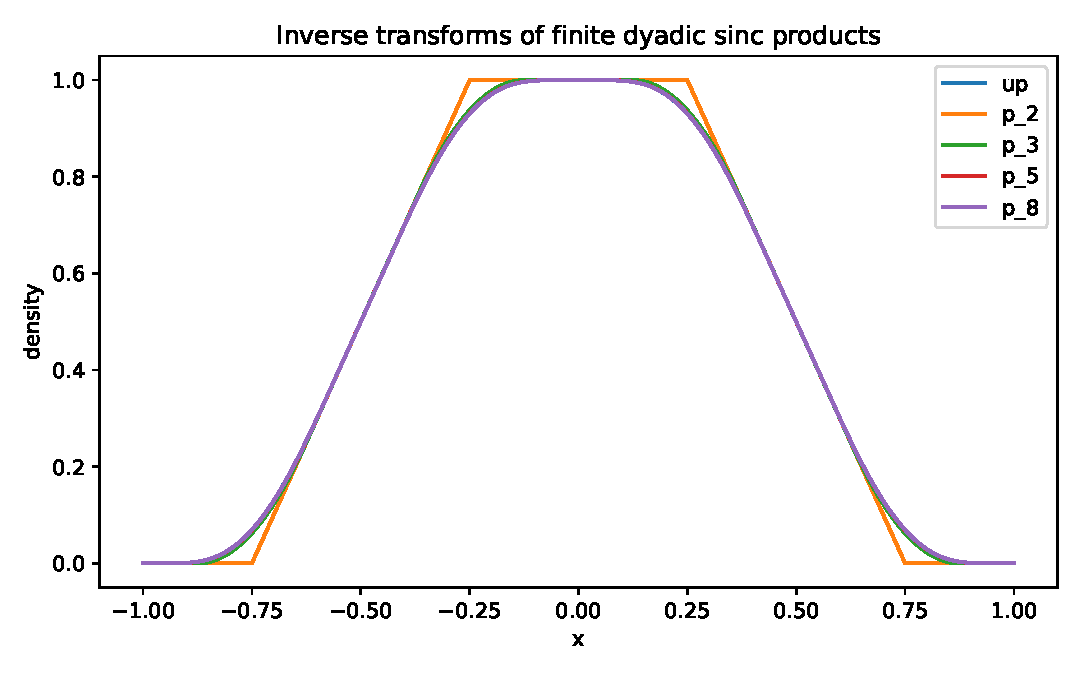
\includegraphics[width=0.88\textwidth]{finite_sinc_approximants.pdf}
\caption{Inverse transforms of the first few finite sinc products.  The support expands
to $[-1,1]$, the polynomial degree and smoothness increase, and the central plateau
shrinks dyadically.}
\label{fig:approximants}
\end{figure}

\begin{figure}[htbp]
\centering
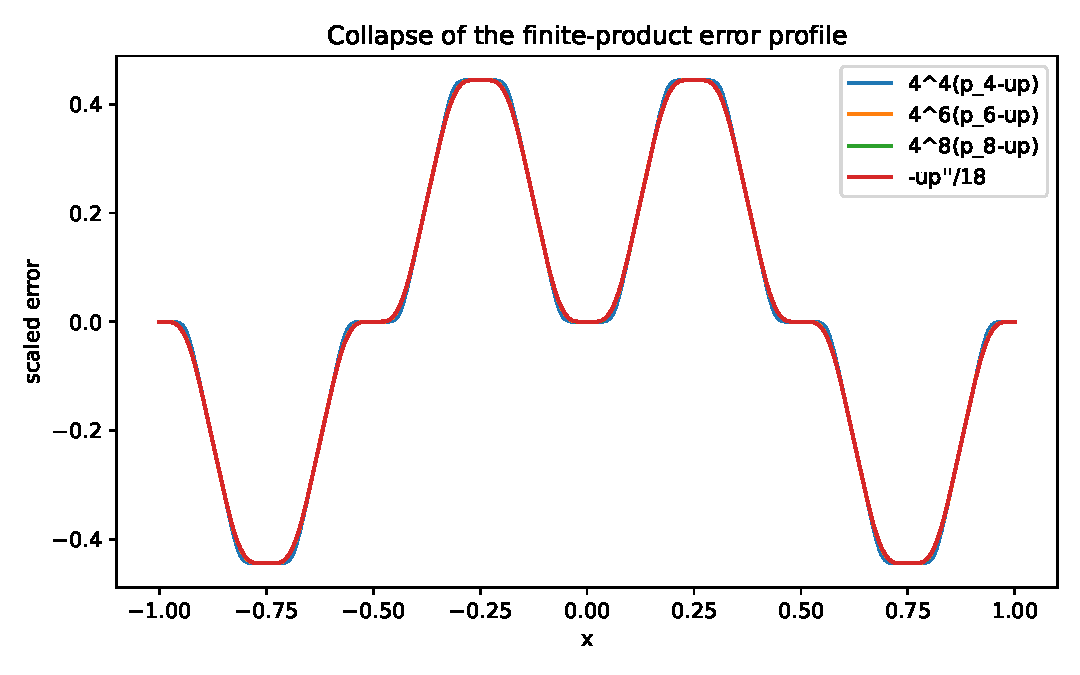
\includegraphics[width=0.88\textwidth]{scaled_error_profiles.pdf}
\caption{The profiles $4^n(p_n-\Up)$ collapse onto $-\Up''/18$, in agreement with
\cref{eq:leading-profile}.}
\label{fig:scaled-errors}
\end{figure}

\begin{figure}[htbp]
\centering
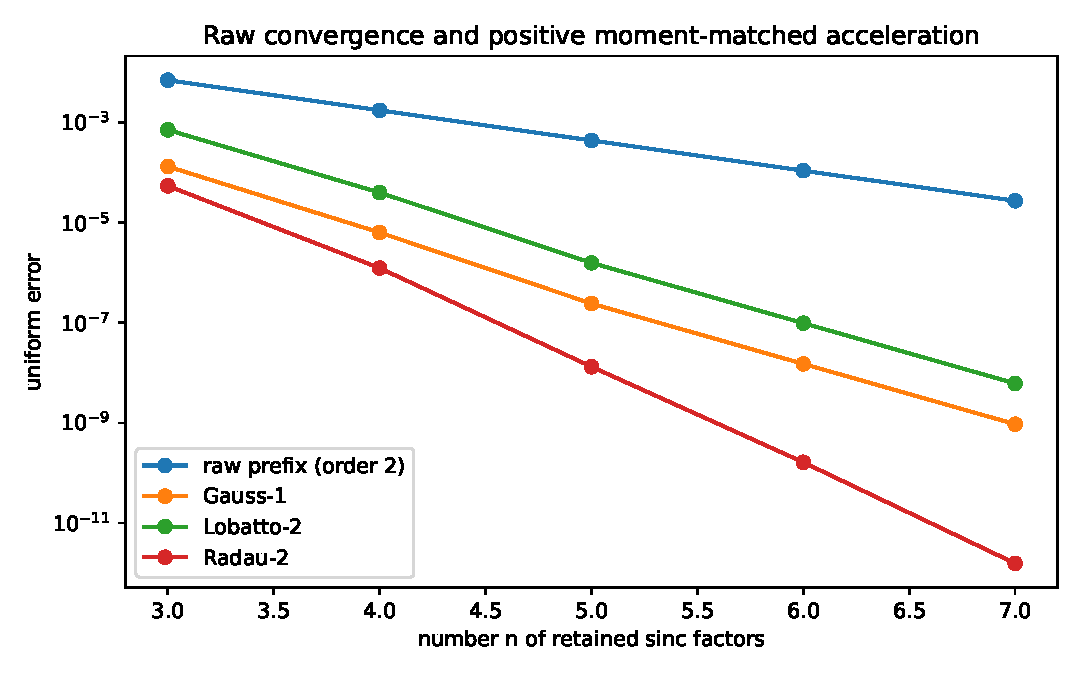
\includegraphics[width=0.88\textwidth]{convergence_comparison.pdf}
\caption{Raw second-order convergence and positive Gauss, Lobatto, and Radau tail
acceleration.  The highest-order Radau values approach the double-precision floor.}
\label{fig:convergence}
\end{figure}

\subsection{Verification of exact constants}

Selected FFT ratios of measured supremum error to the exact formula are shown below.

\begin{center}
\begin{tabular}{@{}lrrrr@{}}
\toprule
Scheme & $r$ & $n$ & measured error & measured/exact\\
\midrule
Raw prefix & 0 & 3 & $6.94444444448\times10^{-3}$ & $1.000000000006$\\
Raw prefix & 2 & 5 & $5.55555555771\times10^{-2}$ & $1.000000000387$\\
Raw prefix & 4 & 7 & $7.11111128754$ & $1.000000024810$\\
Gauss-1 & 0 & 5 & $2.41126543254\times10^{-7}$ & $1.000000000183$\\
Lobatto-2 & 0 & 5 & $1.56732253097\times10^{-6}$ & $1.000000000069$\\
Radau-2 & 0 & 7 & $1.56639950187\times10^{-12}$ & $1.000079775969$\\
\bottomrule
\end{tabular}
\end{center}

The raw and fourth-order laws agree essentially to machine precision.  The Radau error
is already $1.6\times10^{-12}$ at its first admissible $n$, so Fourier truncation and
roundoff visibly affect the last digits.  Full tables are included in
\texttt{sharp\_error\_verification.csv} and
\texttt{positive\_acceleration\_verification.csv}.

\section{Algorithms and implementation considerations}
\label{sec:algorithms}

\subsection{Exact cell construction}

There are three complementary exact representations.

\paragraph{Global truncated powers.}
Equation \cref{eq:truncated-power} evaluates a point in $O(2^n)$ signed rational
operations and is ideal for proof and low-order checks.  Only knots left of $x$ need be
included.

\paragraph{Primitive recursion.}
If a piecewise-polynomial primitive of $p_{n-1}$ is stored cellwise, then
\cref{eq:last-box-recursion} evaluates $p_n$ by two shifted primitive values.  This
constructs the complete spline with exact coefficients while reusing adjacent-cell data.

\paragraph{Top-down integration of the Thue--Morse step.}
Start from the top derivative values in \cref{eq:top-cell-value,eq:tm-prefix}, integrate
cell by cell, and determine constants by continuity and vanishing at the left support
endpoint.  This uses only additions, multiplications by the mesh, and division by small
integers.  It is particularly attractive for formal verification.

\subsection{Positive quadrature construction}

The moment sequence $m_k=(2k+1)\E X^{2k}$ can be generated exactly from the cumulants
\cref{eq:cumulants-X}.  A practical $M$-node Gauss construction is:
\begin{enumerate}[leftmargin=2.1em]
\item compute $m_0,\ldots,m_{2M}$ as rational numbers;
\item perform exact Gram--Schmidt on $1,z,\ldots,z^M$, or solve the Hankel system for
      the monic orthogonal polynomial $P_M$;
\item isolate the $M$ simple roots of $P_M$ in $(0,1)$;
\item solve the Vandermonde moment equations for positive weights;
\item insert the nodes and weights in \cref{eq:gQ-fourier} or
      \cref{eq:gQ-spatial}.
\end{enumerate}
Right-Radau rules are obtained by orthogonalizing against the modified measure
$(1-z)\dd\nu(z)$ and then adjoining $z=1$; Lobatto rules use
$z(1-z)\dd\nu(z)$ and adjoin both endpoints.  Exact rational recurrence coefficients
make certified algebraic output feasible.

\subsection{Numerical stability}

The global formula \cref{eq:truncated-power} contains large alternating terms and should
not be evaluated naively in floating point at high $n$.  Stable options are:
\begin{itemize}[leftmargin=2em]
\item exact rational arithmetic followed by one final conversion;
\item cellwise Horner evaluation after primitive recursion;
\item FFT inversion when values on a dense uniform grid are needed;
\item convolution on adaptive polynomial pieces for positive quadrature mixtures.
\end{itemize}
The Richardson coefficients have uniformly bounded $\ell^1$ norm by
\cref{eq:richardson-stability}; their cancellation is therefore much milder than a
generic high-order extrapolation.  Positive quadrature schemes avoid cancellation
entirely.

\section{Further deductions and research directions}
\label{sec:future}

\subsection{Results that appear immediately accessible}

\begin{problem}[Lean formalization of the prefix law]
Formalize \cref{thm:truncated-power,thm:derivative-plateau,thm:sharp-prefix-law}.
The proof ingredients are already close to the repository's APIs: finite uniform
convolutions, Thue--Morse prefix sums, the exact tail decomposition, bounded weak
second derivatives, and the formally proved sharp derivative tiling of $\Up$.
\end{problem}

\begin{problem}[Certified quadrature generator]
Build an exact-arithmetic pipeline that returns the rational orthogonal polynomial,
certified algebraic nodes, and positive weights for Gauss and right-Radau rules of
$\nu$.  The output would be a library of positive compactly supported approximants with
machine-checkable error constants.
\end{problem}

\begin{problem}[Norms beyond $L^\infty$]
The expansion gives sharp leading constants in every $L^p$ norm.  The exact derivative
distribution identities in the primary exposition suggest that some $L^p$ constants,
rearrangement-invariant norms, or signed error distributions may admit closed forms.
\end{problem}

\subsection{Conjectures}

\begin{conjecture}[$q$-special orthogonal structure]
\label{conj:q-orthogonal}
The monic orthogonal polynomials of
$\dd\nu(z)=-\Up'(\sqrt z)\dd z$ have recurrence coefficients admitting closed
$q$-product or $q$-continued-fraction expressions at $q=1/4$.  Their rationality is
automatic from the rational moments; the conjecture is that the rational numbers have a
simple structural form involving $(q;q)_m$, Gaussian binomials, or the reciprocal-product
coefficients $a_m$.
\end{conjecture}

\begin{conjecture}[Lambert edge scaling of quadrature nodes]
\label{conj:lambert-edge}
The extreme Gauss and Radau nodes have refined endpoint asymptotics controlled by the
same lower-Lambert phase that governs the flat endpoint of the Fabius/Rvachev function.
The leading zero distribution may be classical, but the edge correction should retain
the repository's log-periodic dyadic phase.
\end{conjecture}

\begin{conjecture}[Positive minimax tail rule]
\label{conj:minimax}
Among positive $M$-component uniform scale mixtures supported in $[-1,1]$ and required
to include the endpoint scale $1$, the right-Radau rule minimizes the first nonzero
worst-case $C^r$ error constant simultaneously for all fixed $r$.  The exact plateau
formula reduces this to an extremal moment problem on $[0,1]$.
\end{conjecture}

\begin{conjecture}[Shape preservation]
For every right-Radau rule of $\nu$ and every sufficiently large $n$, the accelerated
density $g_{n,Q}$ is strictly decreasing on $(0,1)$ and has no spurious interior
oscillation.  Positivity is automatic, but monotonicity of a finite mixture is not; a
proof may follow from total positivity of the uniform-box kernel.
\end{conjecture}

\subsection{Broader extensions}

\paragraph{Other geometric bases.}
For $0<q<1$, infinite products generated by widths $(1-q)q^j$ have the same exact
head--tail scaling.  The Bell--Bernoulli expansion and positive tail quadrature survive.
The dyadic case $q=1/2$ is exceptional because subset sums form a uniform grid and the
top derivative is exactly Thue--Morse.  Determining the sharp $C^r$ constants for
general $q$ is a natural next problem.

\paragraph{Multivariate box splines.}
Products of directional sinc factors invert to multivariate box splines.  A geometric
infinite product produces a compactly supported $C^\infty$ atomic function, and finite
prefixes again provide polynomial approximants.  Positive quadrature of the tail scale
may extend with radial or matrix-valued moments.

\paragraph{Inverse Fabius propagation.}
On compact subintervals where $\Up$ is bounded away from zero, the exact error expansion
can be transported through inverse-function calculus to obtain high-order approximations
of the inverse Fabius function.  Near the flat endpoint, the algebraic prefix expansion
must be matched with the Lambert--$W$ asymptotic already developed in the repository.

\paragraph{Spectral and sampling questions.}
The zero multiplicities \cref{eq:zero-multiplicity} suggest dyadic Strang--Fix-type
conditions, multiresolution reconstruction formulas, and exact cancellation identities
for sampled derivatives.  The finite splines could serve as compactly supported
preconditioners whose approximation order is enhanced by the positive tail rules.

\section{Conclusion}

The inverse Fourier transforms of finite dyadic sinc products are much more rigid than
generic finite convolutions.  Binary subset sums force a uniform knot grid; Thue--Morse
signs govern the top derivative; and a precise derivative plateau survives every later
convolution.  Combined with the exact self-similar tail of the Rvachev distribution,
this local geometry turns a Taylor bound into an equality and yields the sharp law
\[
 \norm{p_n^{(r)}-\Up^{(r)}}_\infty
 =\frac{2^{\binom{r+3}{2}-1}}{9\,4^n}.
\]
The same mechanism converts one-signed quadrature errors into exact functional errors.
The resulting Gauss--Radau--Lobatto hierarchy supplies positive piecewise-polynomial
approximants of arbitrary order, with explicit constants and exact support whenever a
right endpoint node is included.  This closes the repository's variance-matched
$16^{-n}$ frontier and opens a tractable new interface among dyadic harmonic analysis,
Thue--Morse combinatorics, Bell--Bernoulli series, orthogonal polynomials, and certified
numerical approximation.

\appendix

\section{Proof of the scale-derivative identity}
\label{app:Ah}

For completeness, we prove \cref{eq:Ah-derivative}.  The case $\ell=0$ is the
definition.  Assume it holds at order $\ell$.  Differentiating under the integral and
using $\partial_z h^{(2\ell)}(\sqrt z u)
=u h^{(2\ell+1)}(\sqrt z u)/(2\sqrt z)$ gives
\[
 A_h^{(\ell+1)}(z)
 =\frac{1}{2^{2\ell+2}\ell!\sqrt z}
 \int_{-1}^{1}u(1-u^2)^\ell h^{(2\ell+1)}(\sqrt z u)\dd u.
\]
Since
\[
 \frac{\dd}{\dd u}(1-u^2)^{\ell+1}
 =-2(\ell+1)u(1-u^2)^\ell,
\]
integration by parts has no boundary term and yields
\[
 A_h^{(\ell+1)}(z)
 =\frac{1}{2^{2\ell+3}(\ell+1)!}
 \int_{-1}^{1}(1-u^2)^{\ell+1}h^{(2\ell+2)}(\sqrt z u)\dd u.
\]
This is the desired induction step.  The formula extends continuously to $z=0$ by
Taylor expansion.

\section{Reproducibility manifest}
\label{app:manifest}

The archive accompanying this report contains:
\begin{itemize}[leftmargin=2em]
\item \path{finite_sinc_products_report.tex} -- the complete source;
\item \path{finite_sinc_products_report.pdf} -- the rendered report;
\item \path{finite_sinc_experiments.py} -- documented numerical and exact code;
\item \path{finite_sinc_approximants.pdf} -- generated approximation figure;
\item \path{scaled_error_profiles.pdf} -- generated error-profile figure;
\item \path{convergence_comparison.pdf} -- generated convergence figure;
\item \path{sharp_error_verification.csv} -- raw-prefix numerical table;
\item \path{positive_acceleration_verification.csv} -- accelerated numerical table;
\item \path{exact_coefficients.txt} -- exact series and Richardson coefficients;
\item \path{exact_rational_samples.csv} -- exact rational spline samples.
\end{itemize}
Run
\begin{lstlisting}[style=reportcode,language=bash]
python finite_sinc_experiments.py --output-dir . --fft-power 17
\end{lstlisting}
to regenerate every figure and table.

\begin{thebibliography}{99}

\bibitem{proveit-primary}
V.~Reshetnikov,
\newblock \emph{The Fabius Function and Rvachev's Up-Function: Exact arithmetic,
probability, Fourier analysis, and corrected sharp asymptotics},
\newblock living TeX exposition in the \texttt{ProveIt} repository, snapshot examined
28 August 2026,
\newblock \url{https://github.com/VladimirReshetnikov/ProveIt/tree/main/Analysis/FabiusFunction/docs/Fabius_Function_and_Rvachev_Up}.

\bibitem{proveit-frontiers}
V.~Reshetnikov,
\newblock \emph{Non-formalized Research Frontiers},
\newblock living consolidated TeX volume in the \texttt{ProveIt} repository, snapshot
examined 28 August 2026,
\newblock \url{https://github.com/VladimirReshetnikov/ProveIt/tree/main/Analysis/FabiusFunction/docs/non-formalized-research-frontiers}.

\bibitem{proveit-archive}
V.~Reshetnikov,
\newblock \emph{Archive of historical document versions},
\newblock recursive archive index in the \texttt{ProveIt} repository,
\newblock \url{https://github.com/VladimirReshetnikov/ProveIt/tree/main/Analysis/FabiusFunction/docs/archive}.

\bibitem{jessen1935}
B.~Jessen and A.~Wintner,
\newblock Distribution functions and the Riemann zeta function,
\newblock \emph{Transactions of the American Mathematical Society} \textbf{38}
(1935), 48--88.

\bibitem{fabius1966}
J.~Fabius,
\newblock A probabilistic example of a nowhere analytic $C^\infty$-function,
\newblock \emph{Zeitschrift f\"ur Wahrscheinlichkeitstheorie und Verwandte Gebiete}
\textbf{5} (1966), 173--174.

\bibitem{rvachev1971}
V.~L.~Rvachev and V.~A.~Rvachev,
\newblock A certain finite function,
\newblock \emph{Dopovidi Akademii Nauk Ukrains'koi RSR, Series A} (1971),
705--707, 764.

\bibitem{rvachev1990}
V.~A.~Rvachev,
\newblock Compactly supported solutions of functional-differential equations and their
applications,
\newblock \emph{Russian Mathematical Surveys} \textbf{45} (1990), no.~1, 87--120.

\bibitem{arias1982}
J.~Arias de Reyna,
\newblock Definici\'on y estudio de una funci\'on indefinidamente diferenciable de
soporte compacto,
\newblock \emph{Revista de la Real Academia de Ciencias Exactas, F\'isicas y Naturales
de Madrid} \textbf{76} (1982), no.~1, 21--38;
English translation, \emph{An infinitely differentiable function with compact support:
Definition and properties}, arXiv:1702.05442 (2017).

\bibitem{arias2018}
J.~Arias de Reyna,
\newblock Arithmetic of the Fabius function,
\newblock \emph{INTEGERS} \textbf{18} (2018), Article A51;
arXiv:1702.06487.

\bibitem{deboor}
C.~de Boor,
\newblock \emph{A Practical Guide to Splines}, revised edition,
\newblock Springer, New York, 2001.

\bibitem{davis-rabinowitz}
P.~J.~Davis and P.~Rabinowitz,
\newblock \emph{Methods of Numerical Integration}, second edition,
\newblock Academic Press, Orlando, 1984.

\bibitem{gautschi}
W.~Gautschi,
\newblock \emph{Orthogonal Polynomials: Computation and Approximation},
\newblock Oxford University Press, 2004.

\bibitem{allouche-shallit}
J.-P.~Allouche and J.~Shallit,
\newblock \emph{Automatic Sequences: Theory, Applications, Generalizations},
\newblock Cambridge University Press, 2003.

\end{thebibliography}

\end{document}
